
\section{Alloy model}
\begin{lstlisting}
open util/boolean
sig System {
	has : set User,
	creates : set Recommendation,
	accumulates : set Match
}

abstract sig User {
	sends : set InternshipRequest,
	receives : set InternshipRequest,
	gets : set Recommendation,
	isProposed : set Recommendation
}{
	one s : System | this in s.has
}

sig Student extends User {
	has : set Competence,
	joins : set Match
}

sig Competence {}{
	one s : Student | this in s.has
}

sig Company extends User {
	creates : set InternshipAdv
}{}

sig InternshipAdv {
	includes : lone InterviewForm,
	collects : set InternshipRequest,
	isInserted : set Recommendation,
	partecipates : set Match
}{
	one c : Company | this in c.creates
}

sig InternshipRequest {
	isAccepted : Bool
}{
	one adv : InternshipAdv | this in adv.collects
	one sender : User | this in sender.sends
	one receiver : User | this in receiver.receives
}

sig Recommendation {}{
	one receiver :  User | this in receiver.gets
	one proposed : User | this in proposed.isProposed
	one adv : InternshipAdv | this in adv.isInserted
	one s : System | this in s.creates
}

sig Match {
	var status : one MatchmakingStatus,
	gathers : set Feedback
}{
	one s : System | this in s.accumulates
	one adv : InternshipAdv | this in adv.partecipates
	one stud : Student | this in stud.joins
}

enum MatchmakingStatus{
	CONTACT_CREATED, INTERVIEW_SET, INTERVIEW_COMPLETED, INTERNSHIP_ACCEPTED, INTERNSHIP_DECLINED, INTERNSHIP_FIRST_HALF, INTERNSHIP_COMPLETED
}

sig InterviewForm {}{
	one adv : InternshipAdv | this in adv.includes
}

sig Feedback {
	direction : FeedbackDirection,
	status : one MatchmakingStatus
}{
	one m : Match | this in m.gathers
}

enum FeedbackDirection{
	S2C, C2S
}


//----------------------------FACTS----------------------------
fact UniqueSystem {
	#System = 1
}
//InternshipRequest
//check that InternshipRequest are c->s or s->c
fact NOInternshipRequest_C2C {
	no req : InternshipRequest, c1 : Company, c2 : Company |
		(req in c1.sends and req in c2.receives)
}
fact NOInternshipRequest_S2S {
	no req : InternshipRequest,  s1 : Student, s2 : Student |
		(req in s1.sends and req in s2.receives)
}

//The adv inside the internship request is created by the company that sends (or receives) that internship request 
fact InternshipRequest_C_owns_Adv {
	all req : InternshipRequest, c : Company, adv : InternshipAdv |
		(req in adv.collects and (req in c.sends or req in c.receives)) implies (adv in c.creates)
}

//There are not multiple internship request with the same fields
fact UniqueInternshipRequest{
	all u_sender : User, u_reciver : User, adv : InternshipAdv | no disj req1, req2 : InternshipRequest |
		(req1 in u_sender.sends and req1 in u_reciver.receives and req1 in adv.collects and 
		req2 in u_sender.sends and req2 in u_reciver.receives and req2 in adv.collects)
}
//There are not bidirectional request (a student S1 to a company C1 and C1 to S1)
fact NoBidirectionalInternshipRequest{
	all req1 : InternshipRequest, req2 : InternshipRequest , u_sender : User, u_reciver : User, adv : InternshipAdv |
		(req1 in u_sender.sends and req1 in u_reciver.receives and req1 in adv.collects) 
		implies not
		(req2 in u_sender.receives and req2 in u_reciver.sends and req2 in adv.collects)
}

//Recommendation
//Recommendation can not be company2company or student2student
fact NORecommendation_C2C {
	no reco : Recommendation, c1 : Company, c2 : Company |
		(reco in c1.isProposed and reco in c2.gets)
}
fact NORecommendation_S2S {
	no reco : Recommendation,  s1 : Student, s2 : Student |
		(reco in s1.isProposed and reco in s2.gets)
}

//The adv inside the recommendation is created by the company that gets (or is proposed in) that recommendation 
fact Recommendation_C_owns_Adv {
	all reco : Recommendation, c : Company, adv : InternshipAdv |
		(reco in adv.isInserted and (reco in c.isProposed or reco in c.gets)) implies (adv in c.creates)
}

//There are not multiple recommendation with the same fields
fact UniqueRecommendation{
	all u_proposed : User, u_getter : User, adv : InternshipAdv | no disj reco1, reco2 : Recommendation |
		(reco1 in u_proposed.isProposed and reco1 in u_getter.gets and reco1 in adv.isInserted and 
		reco2 in u_proposed.isProposed and reco2 in u_getter.gets and reco2 in adv.isInserted)
}

//Match
//There are not multiple match with the same fields
fact CreateUniqueMatchPerRequest {
    	all s : Student, adv : InternshipAdv, req : InternshipRequest | 
		((req in s.sends or req in s.receives) and req in adv.collects and req.isAccepted in True)
       		implies one m : Match |
            	(m in s.joins and m in adv.partecipates)
}
fact CreateUniqueMatchPerRequest2 {
    	all m : Match, s : Student, adv : InternshipAdv | 
		(m in s.joins and m in adv.partecipates)
		implies one req : InternshipRequest |
		((req in s.sends or req in s.receives) and req in adv.collects and req.isAccepted in True)
}
fact UniqueMatch{
	all s : Student, adv : InternshipAdv | no disj m1, m2 : Match |
		(m1 in s.joins and  m1 in adv.partecipates and 
		m2 in s.joins and m2 in adv.partecipates)
}

//State Machine for successful match (will lead to a internship)
pred MatchProgress[m : Match]{
	m.status = CONTACT_CREATED  and eventually (m.status = INTERVIEW_SET)
		and always(m.status = INTERVIEW_SET implies eventually m.status = INTERVIEW_COMPLETED
			and always(m.status = INTERVIEW_COMPLETED implies eventually m.status = INTERNSHIP_ACCEPTED
				and always (m.status = INTERNSHIP_ACCEPTED implies eventually (m.status = INTERNSHIP_FIRST_HALF)
					and always (m.status = INTERNSHIP_FIRST_HALF implies eventually m.status = INTERNSHIP_COMPLETED
						and always (m.status = INTERNSHIP_COMPLETED implies always m.status = INTERNSHIP_COMPLETED)
					)
				)
			)
		)
}

//State Machine for unsuccessful match (will not lead to a internship)
pred MatchProgressDeclined[m : Match]{
	m.status = CONTACT_CREATED  and eventually (m.status = INTERVIEW_SET)
		and always(m.status = INTERVIEW_SET implies eventually m.status = INTERVIEW_COMPLETED
			and always(m.status = INTERVIEW_COMPLETED implies eventually m.status = INTERNSHIP_DECLINED
				and always (m.status = INTERNSHIP_DECLINED implies always m.status = INTERNSHIP_DECLINED)))
}

//InterviewForm
//An interview cannot occour without an InterviewForm
fact NoInterviewWithoutForm {
	all m : Match, adv : InternshipAdv |
		(m in adv.partecipates and m.status = INTERVIEW_SET) implies one form : InterviewForm | form in adv.includes 
}

//Feedback
//There are not multiple feedback with the same fields
fact UniqueFeedback {
	all m: Match | no disj f1, f2 : Feedback | (f1 in m.gathers and f2 in m.gathers and f1.status = f2.status and f1.direction = f2.direction)
}
//Feedback cannot be write in INTERVIEW_SET, INTERNSHIP_ACCEPTED or INTERNSHIP_DECLINED status
fact ImpossibleFeedbackStatus {
	no f : Feedback | f.status = CONTACT_CREATED or f.status = INTERVIEW_SET or f.status = INTERNSHIP_ACCEPTED or  f.status = INTERNSHIP_DECLINED
}

//Feedback cannot be write in status that will be reached in the future
fact NoFeedbackFutureState {
	all m : Match |
		((m.status = INTERNSHIP_COMPLETED and #m.gathers > 0 ) implies all f : m.gathers |  (f.status = INTERVIEW_COMPLETED or f.status = INTERNSHIP_FIRST_HALF or f.status = INTERNSHIP_COMPLETED))
		and
		((m.status = INTERNSHIP_FIRST_HALF and #m.gathers > 0 ) implies all f : m.gathers |  (f.status = INTERVIEW_COMPLETED or f.status = INTERNSHIP_FIRST_HALF))
		and
		(((	m.status = INTERVIEW_COMPLETED 
			or m.status = INTERNSHIP_ACCEPTED 
			or m.status = INTERNSHIP_DECLINED ) and #m.gathers > 0 ) implies all f : Feedback | f in m.gathers and f.status = INTERVIEW_COMPLETED)
		and
		(m.status = INTERVIEW_SET or m.status = CONTACT_CREATED) implies m.gathers = none
}
fact NoFeedbackFutureState2 {
	all f : Feedback |
		((f.status = INTERVIEW_COMPLETED) implies one m : Match | f in m.gathers and (m.status = INTERVIEW_COMPLETED or m.status = INTERNSHIP_ACCEPTED or m.status = INTERNSHIP_DECLINED or m.status = INTERNSHIP_FIRST_HALF or m.status = INTERNSHIP_COMPLETED))
		and
		((f.status =  INTERNSHIP_FIRST_HALF) implies one m : Match | f in m.gathers and (m.status = INTERNSHIP_FIRST_HALF or m.status = INTERNSHIP_COMPLETED))
		and
		((f.status = INTERNSHIP_COMPLETED) implies one m : Match | f in m.gathers and  m.status = INTERNSHIP_COMPLETED)
}
//----------------------------ASSERTION----------------------------
//Check that the maximum number of feedback linked to a match cannot be over 6 (3 possible states and 2 direction for each)
assert moreThan6FeedbackPerMatch {
	all m : Match | #m.gathers < 7}


\end{lstlisting}
\clearpage
\subsection{Example}

\subsubsection{Base World}
\begin{lstlisting}
pred baseWorld {
	//Student
	#Student = 1
	#Competence = 0
	//Company
	#Company = 1
	#InternshipAdv = 1
	//S&C
	#Recommendation = 0
	#InternshipRequest = 0
	#Match = 0
	#Feedback = 0
}
run baseWorld for 6
\end{lstlisting}

\begin{figure}[h]
    \centering
    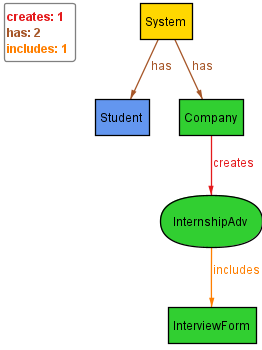
\includegraphics[width=0.5\textwidth]{Images/AlloyModel_images/baseWorld.png}
    \caption{baseWorld}
    \label{fig:figure2}
\end{figure}
Example of the simplest (initial) structure with only one Student and one Company which created an InternshipAdv and an InterviewForm for that ADV.

%------------------------------------------------
\clearpage

\subsubsection{Base World with Recommendation}
\begin{lstlisting}
pred baseWorldWithRecommendation {
	//Student
	#Student = 1
	#Competence = 0
	//Company
	#Company = 1
	#InternshipAdv = 1
	//S&C
	#Recommendation = 1
	#InternshipRequest = 0
	#Match = 0
	#Feedback = 0
}
run baseWorldWithRecommendation for 6
\end{lstlisting}

\begin{figure}[h]
    \centering
    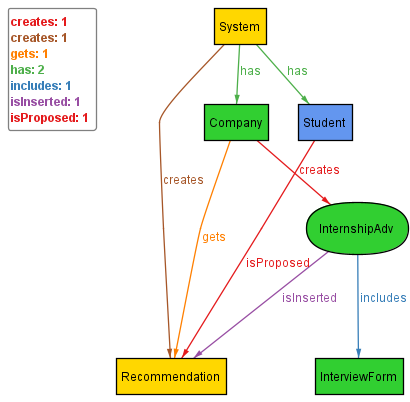
\includegraphics[width=0.75\textwidth]{Images/AlloyModel_images/baseWorldWithRecommendation.png}
    \caption{baseWorldWithRecommendation}
    \label{fig:figure2}
\end{figure}
Example of a structure with only one Student and one Company which created an InternshipAdv and an InterviewForm for that adv. Then the System creates a Recommendation for the Company where a Student is proposed.

%------------------------------------------------
\clearpage

\subsubsection{Base World with Match}
\begin{lstlisting}

pred baseWorldWithMatch {
	//Student
	#Student = 1
	#Competence = 0
	//Company
	#Company = 1
	#InternshipAdv = 1
	//S&C
	#Recommendation = 0
	#Match = 1
	#Feedback = 0
}
run baseWorldWithMatch for 6
\end{lstlisting}

\begin{figure}[h]
    \centering
    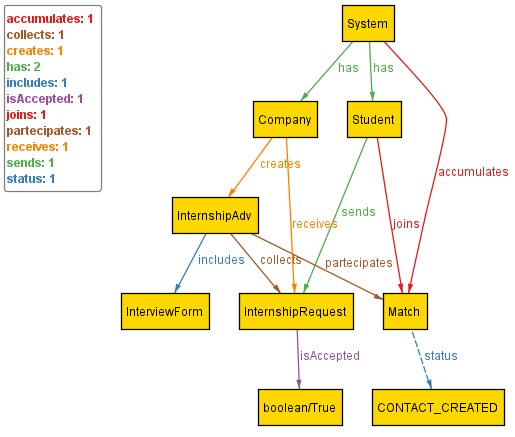
\includegraphics[width=0.8\textwidth]{Images/AlloyModel_images/baseWorldWithMatch.png}
    \caption{baseWorldWithMatch}
    \label{fig:figure2}
\end{figure}
Example of a structure with only one Student and one Company which created an InternshipAdv and an InterviewForm for that adv. The Student sends a InternshipRequest to the Company for the InternshipAdv, the request was accepted (boolean True) so a Match was created and the interview was execute, the status of the Match is INTERNSHIP\_DECLINED.

%------------------------------------------------
\clearpage

\subsubsection{Base World with Match Request Denied}
\begin{lstlisting}
pred baseWorldWithMatchRequestDenied {
	//Student
	#Student = 2
	#Competence = 0
	//Company
	#Company = 1
	#InternshipAdv = 1
	//S&C
	#InternshipRequest = 2
	#Recommendation = 0
	#Match = 1
	#Feedback = 0
}
run baseWorldWithMatchRequestDenied for 6
\end{lstlisting}

\begin{figure}[h]
    \centering
    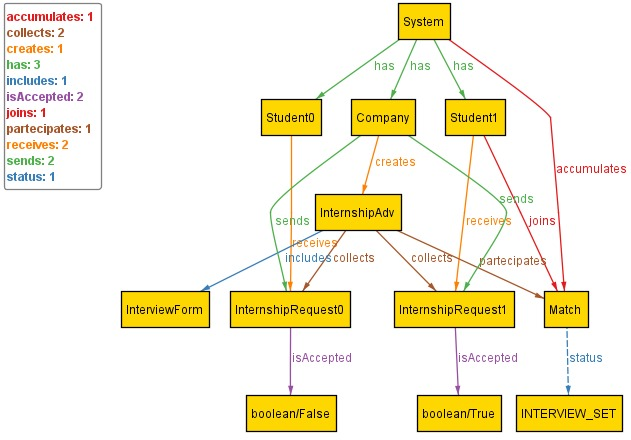
\includegraphics[width=0.9\textwidth]{Images/AlloyModel_images/baseWorldWithMatchRequestDenied.png}
    \caption{baseWorldWithMatchRequestDenied}
    \label{fig:figure2}
\end{figure}
Example of a structure with two Student and one Company which created an InternshipAdv and an InterviewForm for that adv. The Students send an InternshipRequest to the Company for the InternshipAdv, one request was declined (Student0) and one accepted (Student1) so a Match was created.

%------------------------------------------------
\clearpage

\subsubsection{Base World with Feedback}
\begin{lstlisting}
pred baseWorldWithFeedbacks {
	//Student
	#Student = 1
	#Competence = 0
	//Company
	#Company = 1
	#InternshipAdv = 1
	//S&C
	#Recommendation = 0
	#Match = 1
	#Feedback = 4
}
run baseWorldWithFeedbacks for 6
\end{lstlisting}

\begin{figure}[h]
    \centering
    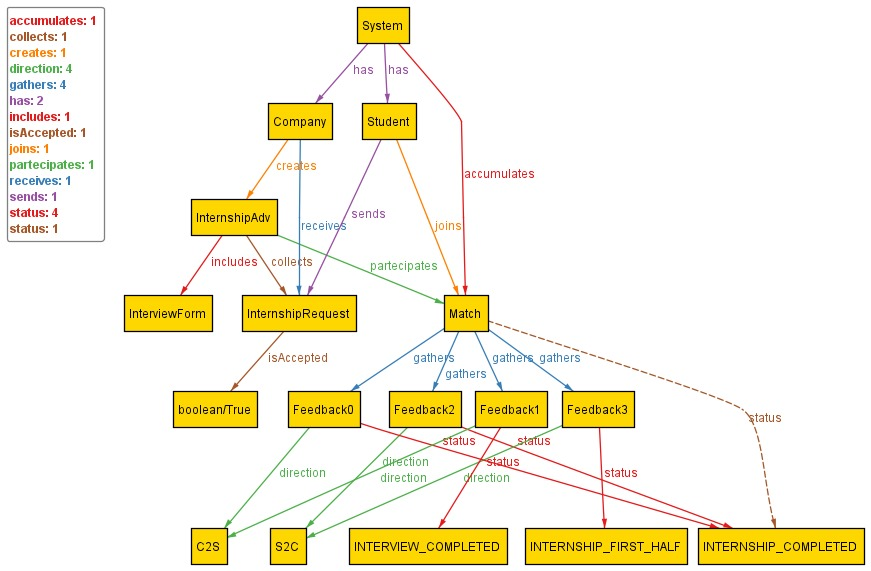
\includegraphics[width=1\textwidth]{Images/AlloyModel_images/WorldWithFeedbacks.png}
    \caption{baseWorldWithFeedbacks}
    \label{fig:figure2}
\end{figure}
Example of a structure with only one Student and one Company which created an InternshipAdv and an InterviewForm for that adv. The Student sends a InternshipRequest to the Company for the InternshipAdv, the request was accepted (boolean True) so a Match was created, the current Status of the Match is INTERNSHIP\_COMPLETED and four Feedbacks were writed: two for the status INTERNSHIP\_FIRST\_HALF (one from Company and one from Student) and the other two for the status INTERNSHIP\_COMPLETED (one from Company and one from Student).\newline

%------------------------------------------------
%\clearpage

\begin{lstlisting}
assert moreThan6FeedbackPerMatch {
	all m : Match | #m.gathers < 7
}
check moreThan6FeedbackPerMatch
\end{lstlisting}

\begin{figure}[h]
    \centering
    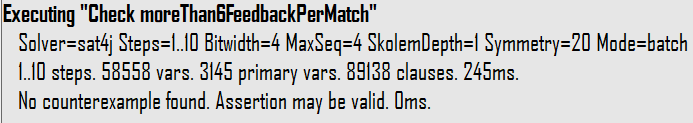
\includegraphics[width=0.8\textwidth]{Images/AlloyModel_images/moreThan6FeedbackPerMatch.png}
    \caption{moreThan6FeedbackPerMatch}
    \label{fig:figure2}
\end{figure}
Assertion to check that the maximum number of feedback linked to a match cannot be over 6 (3 possible states and 2 directions for each).

%------------------------------------------------
\clearpage

\subsubsection{State Machine for Successful Match Evolution}
\begin{lstlisting}
pred SuccessfulMatchEvolution [m : Match] {
	//Student
	#Student = 1
	#Competence = 0
	//Company
	#Company = 1
	#InternshipAdv = 1
	//S&C
	#Recommendation = 0
	#Match = 1
	#Feedback = 0
	MatchProgress[m]
}

run SuccessfulMatchEvolution for 6
\end{lstlisting}

\begin{figure}[h]
    \centering
    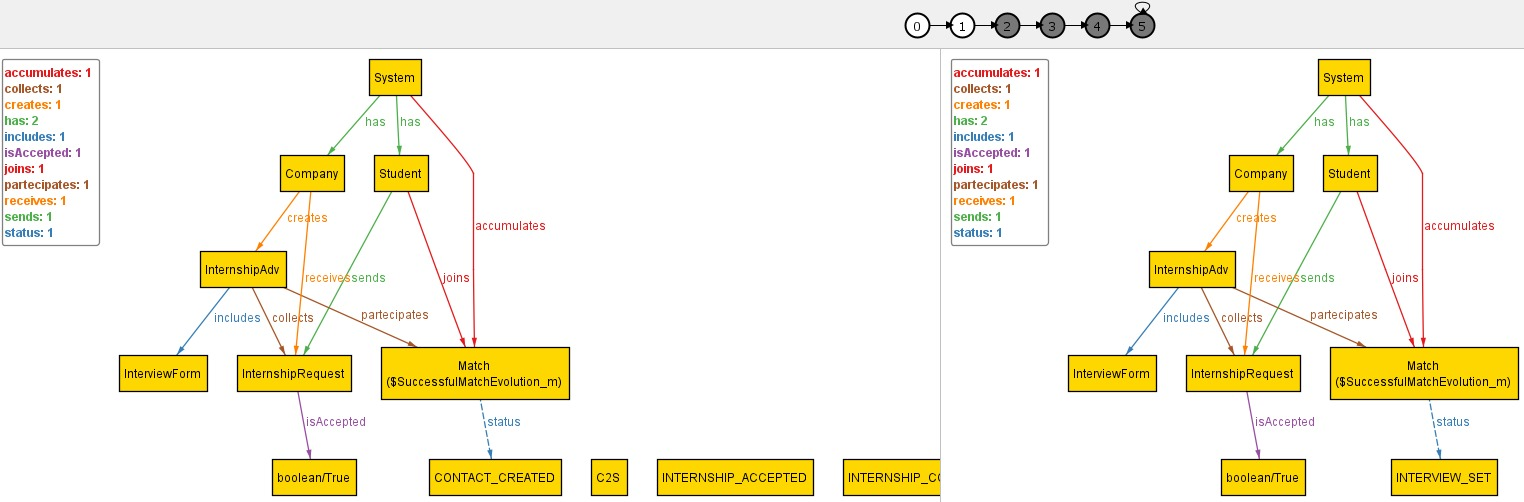
\includegraphics[width=1\textwidth]{Images/AlloyModel_images/SuccessfulMatchEvolution[0-1].png}
    \caption{SuccessfulMatchEvolution[0-1]}
    \label{fig:figure2}
\end{figure}
\begin{figure}[h]
    \centering
    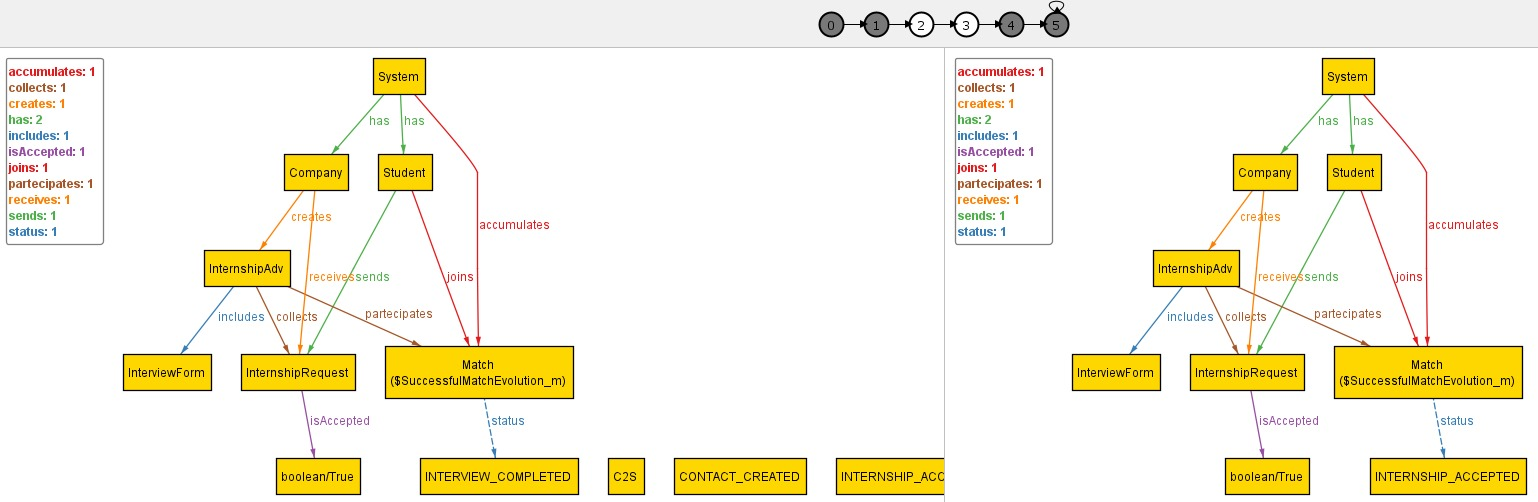
\includegraphics[width=1\textwidth]{Images/AlloyModel_images/SuccessfulMatchEvolution[2-3].png}
    \caption{SuccessfulMatchEvolution[2-3]}
    \label{fig:figure2}
\end{figure}
\begin{figure}[h]
    \centering
    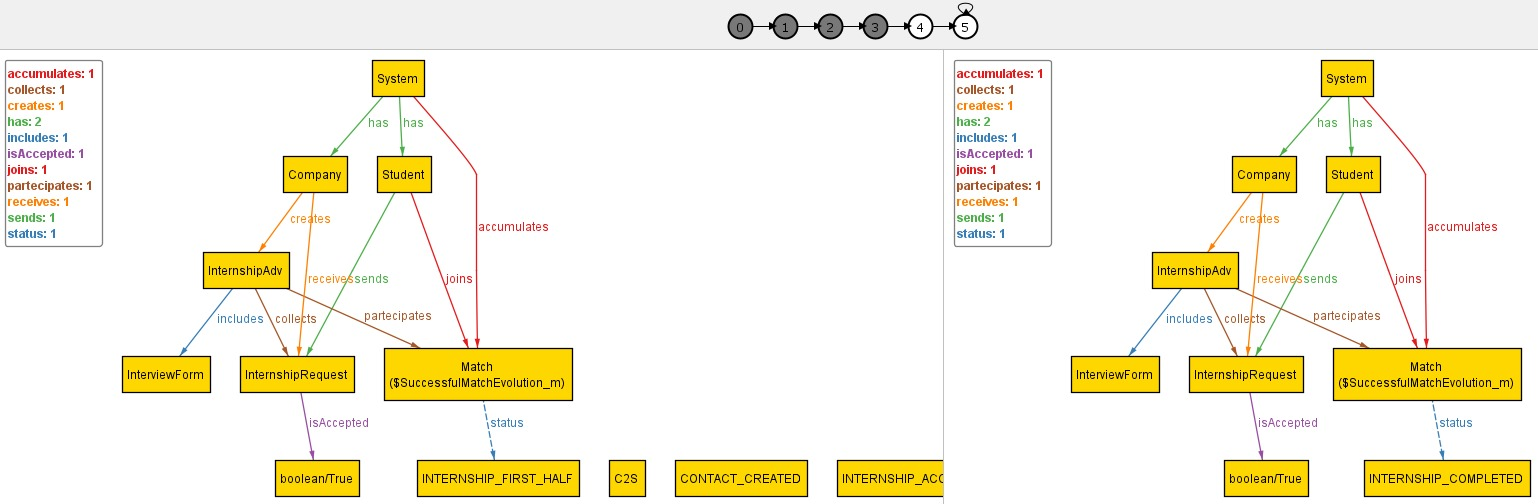
\includegraphics[width=1\textwidth]{Images/AlloyModel_images/SuccessfulMatchEvolution[4-4].png}
    \caption{SuccessfulMatchEvolution[4-4]}
    \label{fig:figure2}
\end{figure}
State machine that describes the behavior of the match Status in a Successful Match Situation (Interview lead to an Internship).

%------------------------------------------------
\clearpage

\subsubsection{State Machine for Unsuccessful Match Evolution}
\begin{lstlisting}
pred UnsuccessfulMatchEvolution [m : Match] {
	//Student
	#Student = 1
	#Competence = 0
	//Company
	#Company = 1
	#InternshipAdv = 1
	//S&C
	#Recommendation = 0
	#Match = 1
	#Feedback = 0
	MatchProgressDeclined[m]
}

run UnsuccessfulMatchEvolution for 6
\end{lstlisting}

\begin{figure}[h]
    \centering
    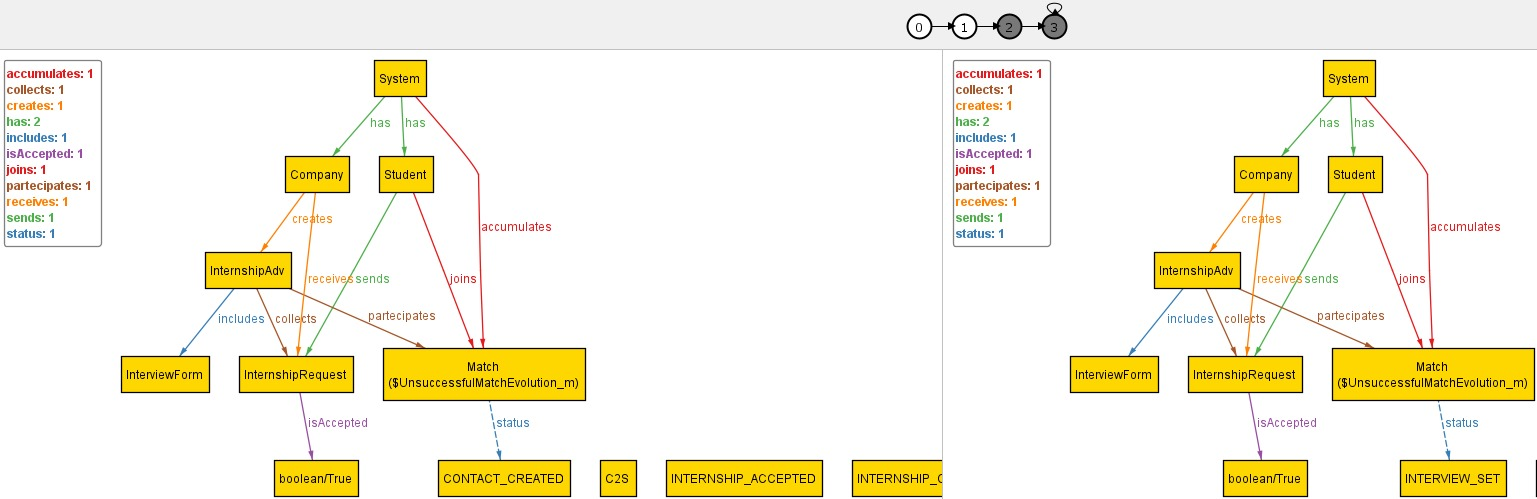
\includegraphics[width=0.85\textwidth]{Images/AlloyModel_images/UnsuccessfulMatchEvolution[0-1].png}
\caption{UnsuccessfulMatchEvolution[0-1]}
    \label{fig:figure2}
\end{figure}
\begin{figure}[h]
    \centering
    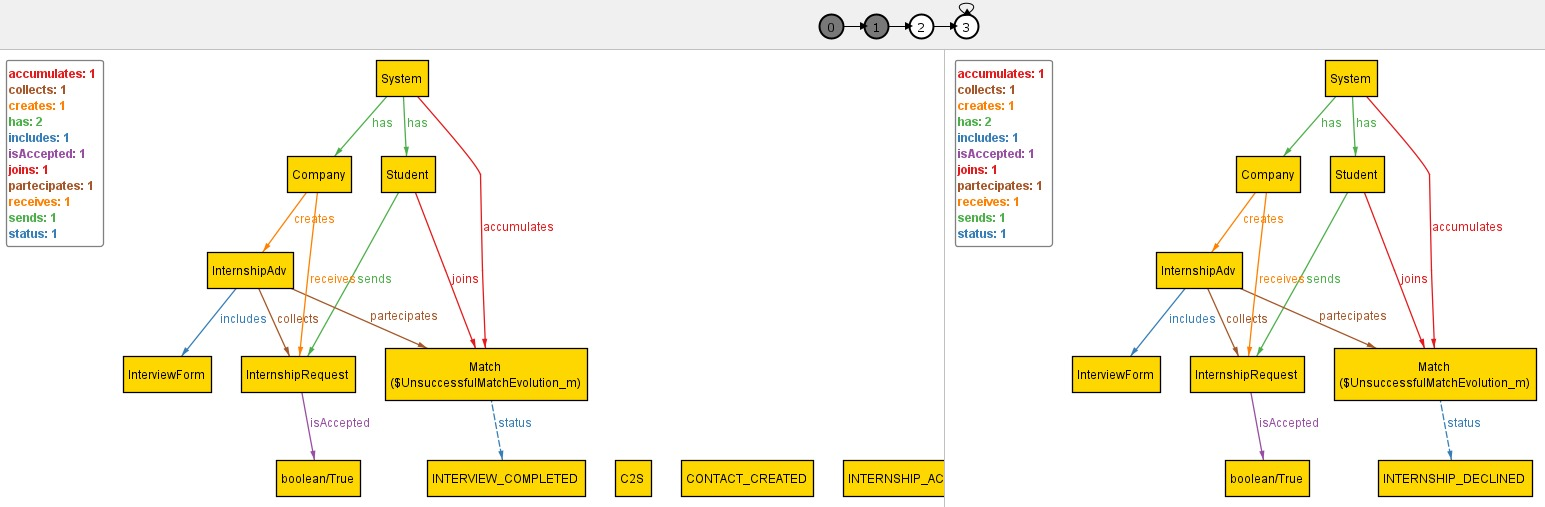
\includegraphics[width=0.85\textwidth]{Images/AlloyModel_images/UnsuccessfulMatchEvolution[2-2].png}
    \caption{UnsuccessfulMatchEvolution[2-2]}
    \label{fig:figure2}
\end{figure}
State machine that describes the behavior of the match Status in a Unsuccessful Match Situation (Interview do not lead to an Internship).

%------------------------------------------------
\clearpage

\subsubsection{Big World}
\begin{lstlisting}
pred BigWorld {
	//Student
	#Student = 2
	#Competence = 1
	//Company
	#Company = 2
	#InternshipAdv = 1
	//S&C
	#Recommendation = 0
	#Match = 2
	#Feedback = 1
}

run BigWorld for 6
\end{lstlisting}

\begin{figure}[h]
    \centering
    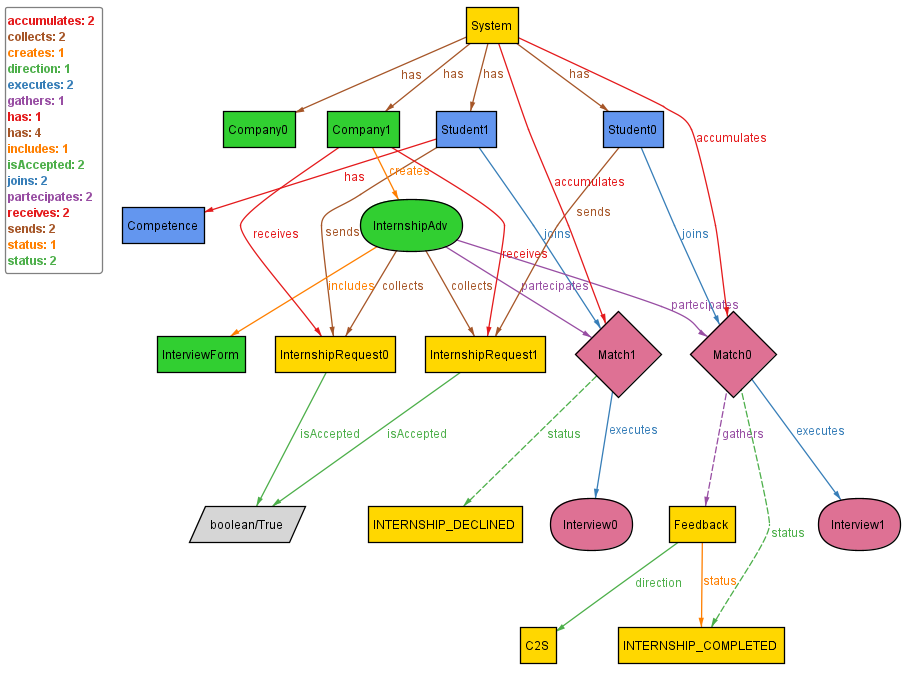
\includegraphics[width=1\textwidth]{Images/AlloyModel_images/BigWorld.png}
    \caption{BigWorld}
    \label{fig:figure2}
\end{figure}
Example of a more complex structure with multiple Students and Companies, which interact with each other creating InternshipRequest, Match and writing Feedback.
